%!TEX TS-program = lualatex
%!TEX encoding = UTF-8 Unicode

\documentclass[final,hyperref={pdfpagelabels=false}]{beamer}
% Width and height in cm
\usepackage[size=custom, width=111.7, height=91.4, orientation=landscape, debug, scale=1.4]{beamerposter}

%\usepackage{graphicx}
%	\graphicspath{{img/}}

	
\usepackage{fontspec}
\def\mainfont{Linux Biolinum O}
\setmainfont[Ligatures={Common,TeX}, Contextuals={NoAlternate}, BoldFont={* Bold}, ItalicFont={* Italic}, Numbers={OldStyle}]{\mainfont}
\setsansfont[Ligatures={Common,TeX}, Scale=MatchLowercase, Numbers=OldStyle]{Linux Biolinum O} 
\usepackage{microtype}

\usepackage{unicode-math}
%\setmathfont[Scale=MatchLowercase]{Asana Math}
%\setmathfont[Scale=MatchLowercase]{XITS Math}

\usepackage[absolute,overlay]{textpos}

\usepackage{natbib}
%\setlength{\leftmargini}{0.9em}

\settowidth{\leftmargini}{\usebeamertemplate{itemize item}}
\addtolength{\leftmargini}{\labelsep}

\AtBeginDocument{%
	\abovedisplayskip=12pt plus 3pt minus 9pt
	\abovedisplayshortskip=-0.5\baselineskip
	\belowdisplayskip=12pt plus 3pt minus 9pt
	\belowdisplayshortskip=0.5\baselineskip
}
\newcommand{\whitespace}{\vspace{0.5\baselineskip}}

\mode<presentation>{
	\usetheme{SEMO}
}

% This idea from the Jacobs landscape poster template 
% http://www.latextemplates.com/cat/conference-posters
\newlength{\sepwid}
\newlength{\onecolwid}
\newlength{\twocolwid}
\newlength{\threecolwid}
\setlength{\sepwid}{0.015\paperwidth} % Separation width (white space) between columns
\setlength{\onecolwid}{0.23\paperwidth} % Width of one column
\setlength{\twocolwid}{0.464\paperwidth} % Width of two columns
\setlength{\threecolwid}{0.7\paperwidth} % Width of three columns


%%%%%%%%%%%%%%%%%%%%%%%%%%%%%%%%%%%%%%%%%%%%%%%%%%%%%%%%%%%%%%%%%%%%%%%%%%%%%%%%%5
\graphicspath{{img/}}
\title[Analysis in the Classroom]{Through the Years: A Quantitative Biology Curriculum}
\author[Taylor]{Michael S. Taylor}
\institute[SEMO]{Department of Biology}
\date{23 July 2017}


%%%%%%%%%%%%%%%%%%%%%%%%%%%%%%%%%%%%%%%%%%%%%%%%%%%%%%%%%%%%%%%%%%%%%%%%%%%%%%%%%5
\begin{document}

% To cite the Vision and Change document.
\defcitealias{national2003bio2010}{\textsc{nrc}, 2003}
\defcitealias{american2011vision}{\textsc{aaas}, 2011}

\begin{frame}[t]
%\vspace{\sepwid}
\begin{columns}[t]
	\begin{column}{\sepwid} % Left spacer
	\end{column}
	\begin{column}{\onecolwid}
    	\begin{block}{Introduction}
    		\textsc{Quantitative reasoning} is a skill that must be mastered by biology students before they graduate \citetext{\citetalias{national2003bio2010}; \citetalias{american2011vision}; \citealp{hurney2011closing}}. Yet, experience suggests that biology students do not always see the need for this skill (“I just want to work with plants.”) or fear analytical problems (“I am not good at math.”). Student aversion to quantitative analysis poses pedagogical problems for teaching the process of science.
    		
    		\whitespace

			To address these problems, some biology faculty at Southeast have coordinated their courses to teach skills early that are built upon later. For example, the first  biology course for majors uses Microsoft Excel extensively to teach fundamental graphing and math functions that students use for data analysis. Later courses require students to employ those early skills and to learn more advanced skills. Some courses introduce new software for simulation and analysis. Here, I highlight exercises from three courses that span the curriculum of a typical organismal biology student at Southeast.  
    	\end{block}

		\vspace*{\sepwid}

		\begin{block}{Literature Cited}
			\setlength{\bibhang}{0.5em}
			\bibliographystyle{amnatnat}
			\raggedright
			{\small \bibliography{modeling_workshop}}
		\end{block}

		\vspace*{0.5\sepwid}
		
		\textcolor{river}{\textbf{\textsc{Colophon}}}
		
			{\justifying\small This poster was typeset with \LaTeX{} and the beamerposter package by Philippe Dreuw and Thomas Deselaers. The font is Linux Biolinum O produced by LinuxLibertine.org. The poster and template are available from mtaylor-semo on github.com  (\textsc{cc by-sa 4.0}).}
		

	\end{column}
	\begin{column}{\sepwid}
	\end{column}
	\begin{column}{\onecolwid}
	    \begin{block}{Year 1: Evolution and Ecology}
    	   	\textsc{Evolution and Ecology} is a new lecture and laboratory course for freshmen biology majors. The lab exercises help students develop skills with Microsoft Excel and emphasize graphical analyses of data.
			
			\whitespace
			
			\textsc{Hardy-Weinberg Equilibrium}
			
			Students use two equations to model allele and genotype frequencies in a population of organisms. The equation for the allele frequencies is
			
			\begin{equation*}
				p + q = 1,
			\end{equation*}
			
			where $p$ and $q$ are the frequencies of two alleles. The formula for the three possible genotypes is
			
			\begin{equation*}
				p^2 + 2pq + q^2 = 1.
			\end{equation*}
						
			Students build formulas in Excel to generate values for the five variables from $p = 0.01$ to $1.0$, and then plot the three genotype frequencies against the $p$ allele frequency. The graph is a visual representation of \textit{expected} genotype frequencies for a population in Hardy-Weinberg equilibrium.
						
			\whitespace

			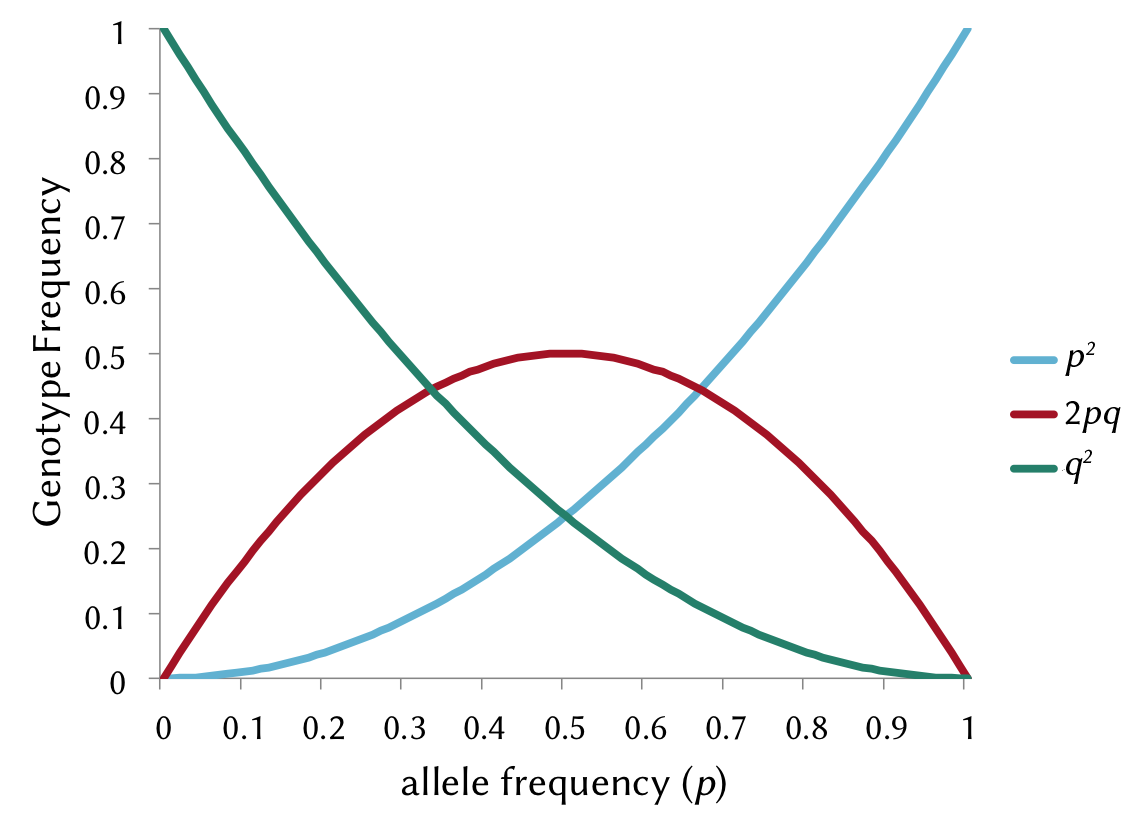
\includegraphics[width=\textwidth]{hwe_graph}
			
			\whitespace
			
			Students next apply “beanbag” biology \citep{jungck2010mathematical} by sampling “alleles” from a “population” with known allele frequencies, and then apply a $\chi^2$ test to compare observed to expected genotype frequencies. Students also explore how migration and natural selection affect allele frequencies in a population.
			
			\whitespace
			
			Representative questions from the migration component are
			
			\begin{itemize}\justifying
				\item Predict how the frequency of each allele will change for each population due to gene  flow.
				
				\item Use the results of your migration simulation to explain why gene flow between populations should prevent them from becoming genetically different.
			\end{itemize}
			
    	\end{block}
	\end{column}

	\begin{column}{\sepwid}
	\end{column}

	\begin{column}{\onecolwid}
    	\begin{block}{Years 2–3: Evolutionary Biology}
       		\textsc{Introduction to Evolutionary Biology} is taken by sophomores and juniors. The course is now lecture-only but is being redesigned to include a once-per-week lab that requires to students to reinforce lecture concepts by analysis of real data.
       		
       		\whitespace
       		
       		\textsc{Population Genetics} 
       		
       		Students use PopG software \citep{Felsenstein2016:popg} to simulate allele frequencies in a population subject to different evolutionary scenarios such as natural selection and genetic drift. With PopG, students change population size, strength of selection, and migration and mutation rates to learn how these affect allele frequencies over time.
       		
       		\whitespace
       		
       		In one exercise, students explore the interaction between the strength of selection $\left(s\right)$ and the effective population size $\left(N_e\right)$:
       		
       		\begin{equation*}
       		2N_es \approx 1.
       		\end{equation*}
       		
       		If $2N_es \gg 1$ then selection has a better chance of overcoming drift to cause a beneficial mutation to become fixed in the population. In a series of simulations where $2N_es = 0$ and $2N_es = 2$, students see that a beneficial allele has about a $4\times$ greater chance of becoming fixed in the population. The figure below shows the results of one simulation run on 100 populations of $N = 100$ each and $s = 0.01$.
       		
			\whitespace

			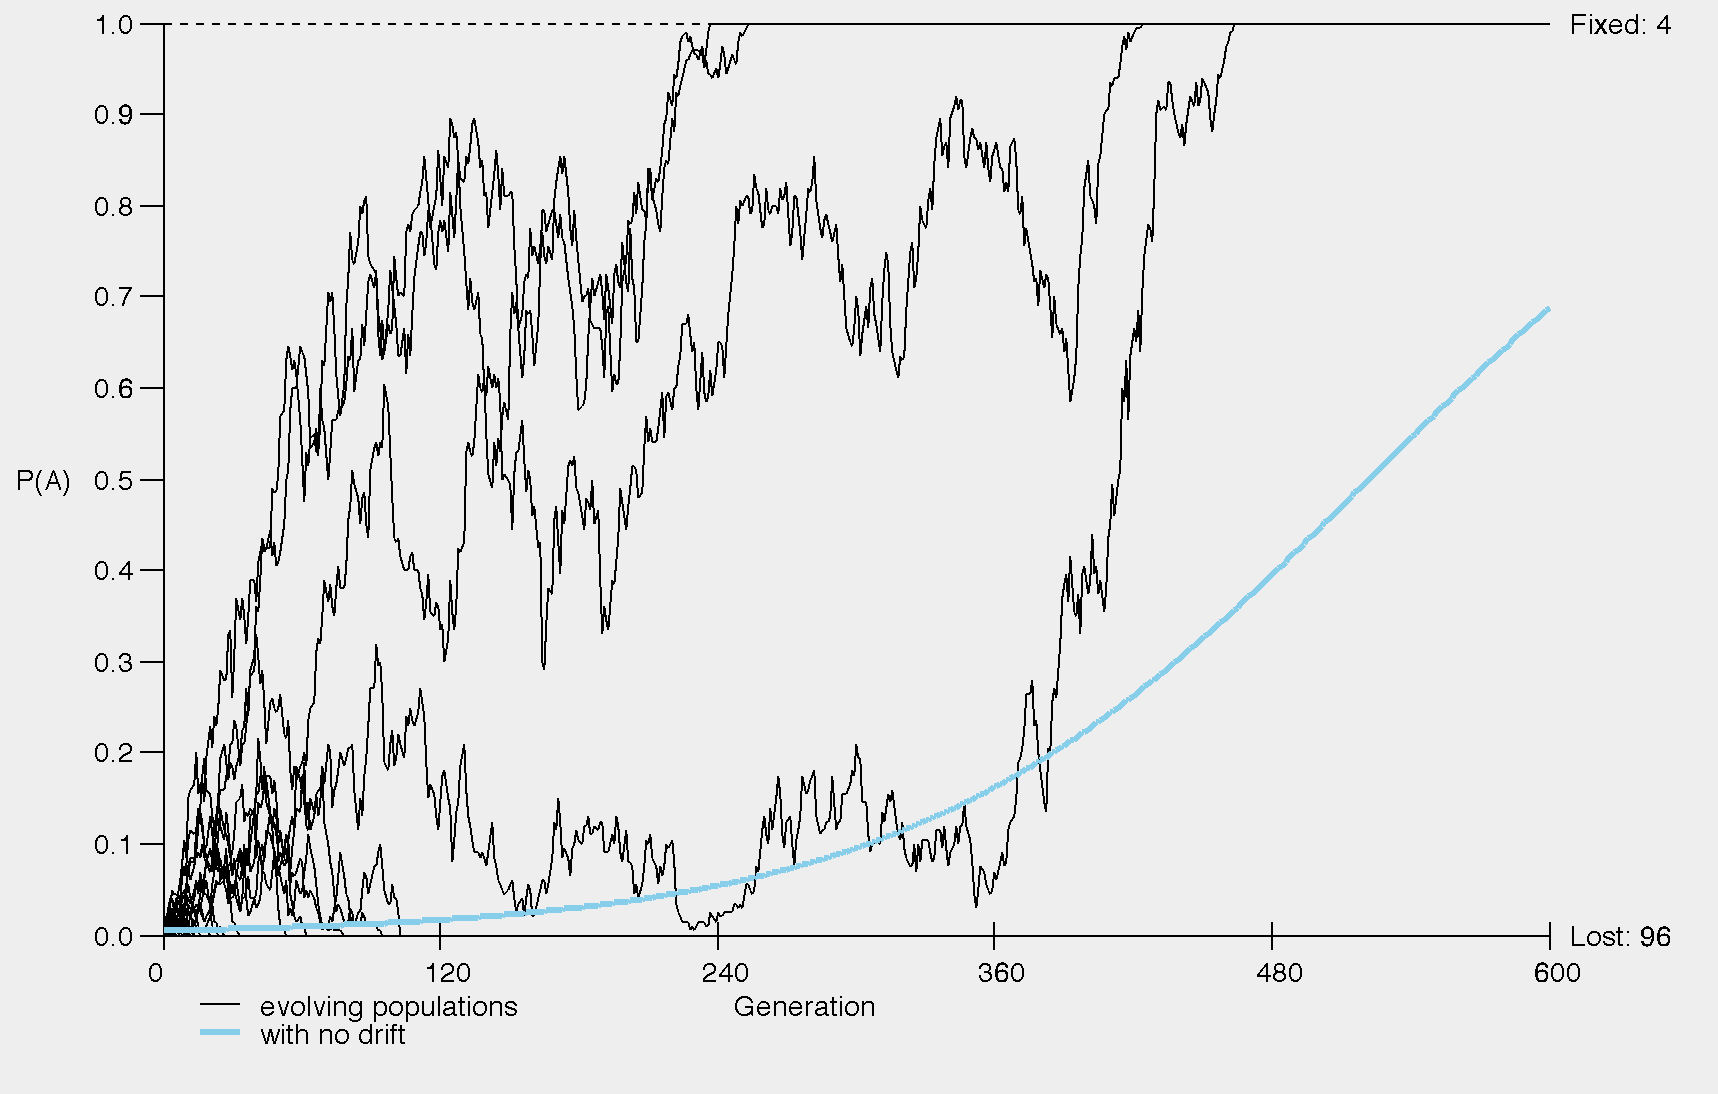
\includegraphics[width=\textwidth]{ns_graph}

			\whitespace
       		
       		Representative questions from this exercise are
       		\begin{itemize}\justifying
       			
       			\item Predict how $N_e$ affects the probability of fixation for an allele under weak positive selection $\left(s = 0.01\right)$. Justify your predictions for populations of $N = 1000$ and $N = 10,000$.
       			
%       			\item Draw a graph that predicts the allele frequency change for starting $p = 0.005$, $N_e = 100$, and relative fitnesses of 1.0, 0.99 and 0.98 for the  \emph{AA}, \emph{Aa} and \emph{aa} genotypes.
       			
       			\item What should be the strength of selection in a population of $N_e = 1000$ to overcome the effects of genetic drift? If $N_e = 10,000$ or $50,000$? Show your work.
       		\end{itemize}
       		
		\end{block}
	\end{column}

	\begin{column}{\sepwid}
	\end{column}

	\begin{column}{\onecolwid}
  	  	\begin{block}{Year 4: Biogeography}
			\textsc{Biogeography} is a senior and graduate level course. Students use the R Statistical Package \citep{R-Core-Team:2016aa} to analyze real-world data to discover and report biogeographic patterns.
			
       		\whitespace

			\textsc{Biogeographic Provinces} 

			Students compare distribution patterns of freshwater fishes and crayfishes by performing a principal coordinates ordination (\textsc{pco}) for each taxonomic group. \textsc{Pco} groups watersheds based on shared species, as shown here for Georgia fishes.
		
			\whitespace

			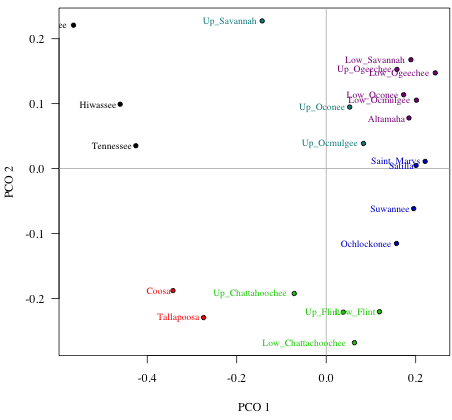
\includegraphics[width=\textwidth]{fishes_pco}

%			\whitespace
			
			Students then compare the similarities of the fish and crayfish ordinations with a Procrustes analysis. A significant result indicate that the watersheds have the same spatial relationship in each ordination, suggesting that fishes and crayfishes share a common biogeographic history. 
			
			\whitespace
			
			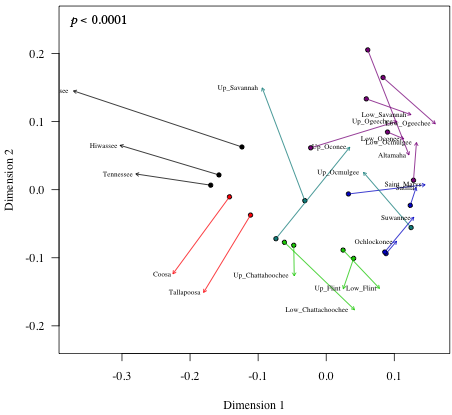
\includegraphics[width=\textwidth]{procrustes}
			
			\whitespace
			
			%Groups of students perform these analyses on pairs of aquatic organisms (mussels, fishes, crayfishs) for different states, and then report their results to the class.
			
		\end{block}
	\end{column}

	\begin{column}{\sepwid}
	\end{column}

	\end{columns}
\end{frame}
\end{document}


%%%%%%%%%%%%%%%%%%%%%%%%%%%%%%%%%%%%%%%%%%%%%%%%%%%%%%%%%%%%%%%%%%%%%%%%%%%%%%%%%%%%%%%%%%%%%%%%%%%%
%%% Local Variables: 
%%% mode: latex
%%% TeX-PDF-mode: t
%%% End:
